\subsection{Mionium v křemíku}	
	Pokud se dostatečně silná vrstva krystalu křemíku bombarduje (anti-)miony $\mu^{+}$, vznikne mionium a naváže se uvnitř krystalové mříže za tvorby šesterečné struktury s okolními atomy.
	Interakce mionia s krystalem se dá modelovat Hamiltoniánem
	\begin{equation}
		\operator{H}'=E_{0}+\frac{A'}{\hbar^{2}}\,\vectoroperator{s}_{\mu}\cdot\vectoroperator{s}_{e}+\frac{D}{\hbar^{2}}\,\operator{s}_{\mu3}\operator{s}_{e3},
	\end{equation}
	což je rozšířený Hamiltonián volného mionia.
	Interakce s mříží je popsána druhým a třetím členem, proto je v obecném případě konstanta $A'$ odlišná od konstanty $A$ pro volné mionium.\footnote{
		Poslední člen v Hamiltoniánu narušuje sférickou symetrii interakce.
		Rotační symetrie okolo osy $z$ však zůstane zachována.
	}
	Konstanty $A'>0$, $D<0$ se určují experimentálně, jejich znaménko je dané.
	
	\begin{enumerate}
	\item 
		Napište matici Hamiltoniánu $\operator{H'}$ a určete její vlastní hodnoty a vlastní stavy.
	
	\item 
		Předpokládejte, že dopadající miony jsou polarizovány do kladného směru osy $x$, tj. $\ket{\psi_{\mu}}=\ket{x+}\hi{\mu}=\ket{\rightarrow}\hi{\mu}$.
		Nalezněte vyjádření počátečního vektoru mionu v bázi $\left\{\ket{\uparrow}\hi{\mu},\ket{\downarrow}\hi{\mu}\right\}$.
		
	\item 
		Předpokládejte, že elektrony jsou před vznikem mionia polarizovány v kladném, resp. záporném směru osy $z$,
		tj. uvažujeme dva případy $\ket{\psi_{e\uparrow}}=\ket{\uparrow}\hi{e}$, $\ket{\psi_{e\downarrow}}=\ket{\downarrow}\hi{e}$.
		Nalezněte stav složeného systému elektron-mion v čase $t=0$, v čase $t$	a pravděpodobnost $p_{\mu\rightarrow}(t)$, že v čase $t$ naměříte spin mionu orientovaný ve směru osy $x$ pro obě dvě počáteční orientace spinu elektronu.
	
	\item 
		Spočítejte totéž jako v předchozím bodu pro případ, že jsou elektrony na počátku
		ve smíšeném stavu
		\begin{equation}
			\operator{\rho}_{e}
				=\frac{1}{2}\ket{\uparrow}\hi{e}\bra{\uparrow}\hi{e}
				+\frac{1}{2}\ket{\downarrow}\hi{e}\bra{\downarrow}\hi{e}\,.
		\end{equation}
		Pravděpodobnost označte $p_{\mu\rightarrow}'(t)$.
	\end{enumerate}

	\begin{figure}[!htbp]
		\centering
		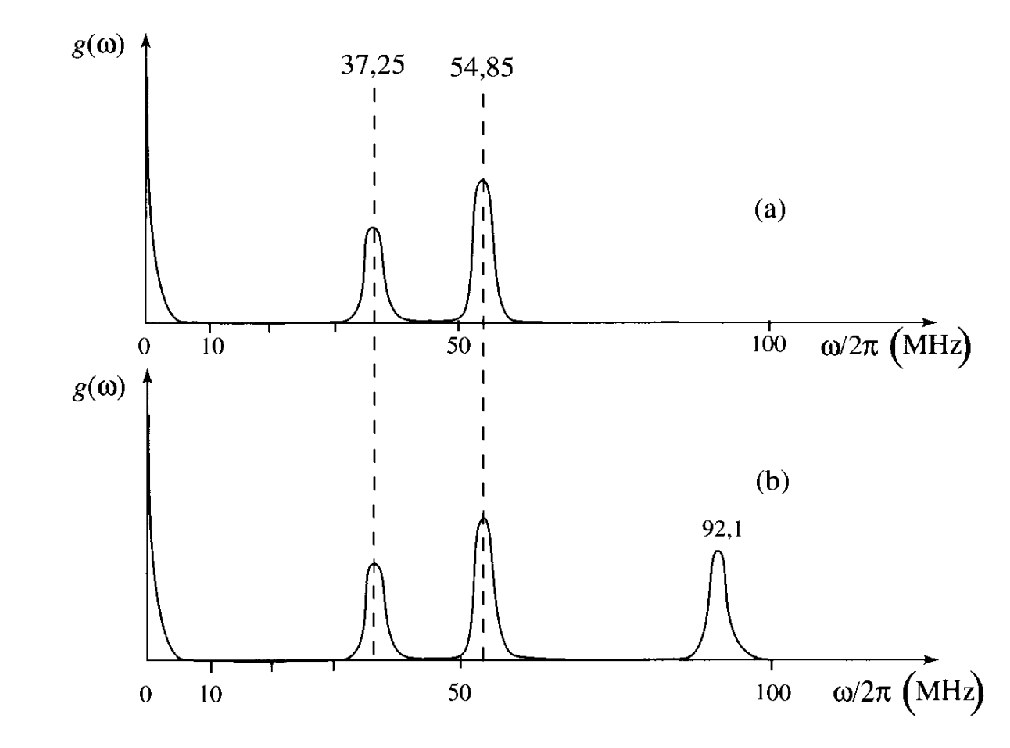
\epsfig{file=figures/mionium.eps,width=0.9\linewidth,keepaspectratio}
		\caption{
			Naměřená funkce $g(\omega)=\real f(\omega)$ pro mionium (převzato z~\cite{Basdevant2000}).
		}
		\label{fig:mionium}
	\end{figure}		

	\subsubsection*{Srovnání s experimentem:}
	Z důvodu konečné doby života se mion v mioniu rozpadá a emituje pozitron $e^{+}$ s největší pravděpodobností ve směru polarizace mionia.
	V praxi se tedy měří směr vylétávajícího pozitronu jako funkce času $t$.
	Při bombardování balíkem $N_{0}$ mionů je počet pozitronů v čase vylétávajících podél osy $x$ 
	\begin{equation}
		\derivative{N(t)}{t}=\frac{N_{0}}{\tau}p_{\mu\rightarrow}(t)\e^{-\frac{t}{\tau}},
	\end{equation}
	přičemž faktor $\frac{1}{\tau}\e^{-\frac{t}{\tau}}$ ve výrazu postihuje exponenciální rozpad mionu se střední dobou $\tau\approx2.2\,\mathrm{\mu s}$.
	Experimentálně se neměří přímo pravděpodobnost $p_{\mu\rightarrow}(t)$, nýbrž tzv. \emph{charakteristická funkce}\index{funkce!charakteristická} $g(\omega)=\real f(\omega)$, kde
	\begin{equation}
		f(\omega)=\frac{1}{\tau}\int_{0}^{\infty}p_{\mu\rightarrow}(t)\e^{-\frac{t}{\tau}}\e^{\im\omega t}\d t
	\end{equation}
	je Fourierova transformace\index{transformace!Fourierova} funkce $\frac{p_{\mu\rightarrow}(t)}{\tau}\e^{-\frac{t}{\tau}}$.
	Příklad naměřené funkce $g(\omega)$ je na obrázku~\ref{fig:mionium}.
			
	\begin{enumerate}
	\setcounter{enumi}{4}
	\item 
		Nalezněte explicitní výraz pro $f(\omega)$ pomocí $f_{0}(\omega)$,
		kde
		\begin{equation}
			f_{0}(\omega)
				\equiv\frac{1}{\tau}\int_{0}^{\infty}\e^{-\frac{t}{\tau}}\e^{\im\omega t}\d t
		\end{equation}	
		je charakteristická funkce volného mionu.
	
	\item
		Z udané hodnoty střední doby života mionu určete, jaká by měla být pološířka vrcholů.
	
	\item
		Z měření zobrazeném na obrázku~\ref{fig:mionium}(a) nalezněte hodnoty parametrů $A'$ a $D$.

	\item
		Na obrázku~\ref{fig:mionium}(b) je totéž měření, jen uspořádání měřícího zařízení bylo lehce pozměněno.
		Diskutujte, k jaké změně v zapojení experimentu došlo.					
	\end{enumerate}

\begin{solution}
	\begin{enumerate}
	\item 
		Matice Hamiltoniánu $\operator{H}'$ vyjádřená v bázi $\mathcal{B}$~\eqref{eq:TwoSpinsBasis} má tvar
		\begin{equation}
			\matrix{H}'=E_{0}+\makematrix{\frac{A'}{4}+D & 0 & 0 & 0 \\ 0 & -\frac{A'}{4}-D & \frac{A'}{2} & 0 \\
				0 & \frac{A'}{2} & -\frac{A'}{4}-D & 0 \\ 0 & 0 & 0 & \frac{A'}{4}+D}
		\end{equation}
		a spektrum po zdiagonalizování je
		\begin{subequations}
			\begin{align}
				E'_{1,4}&=E_{0}+\frac{A'}{4}+D, && 
					\begin{array}{l} \ket{E'_{1}}=\ket{1,1}=\ket{\uparrow\uparrow} \\ \ket{E'_{4}}=\ket{1,-1}=\ket{\downarrow\downarrow} \end{array},\\
				E'_{2}&=E_{0}+\frac{A'}{4}-D, &&
					\ket{E'_{2}}=\ket{1,0}=\frac{1}{\sqrt{2}}\left(\ket{\uparrow\downarrow}+\ket{\downarrow\uparrow}\right),\\
				E'_{3}&=E_{0}-\frac{3A'}{4}-D, && 
					\ket{E'_{3}}=\ket{0,0}=\frac{1}{\sqrt{2}}\left(\ket{\uparrow\downarrow}+\ket{\downarrow\uparrow}\right).
			\end{align}				
		\end{subequations}
		Vlastní vektory jsou tedy totožné jako v případě volného mionia, jediný rozdíl je v tom, že dodatečná interakce řízená parametrem $D$ rozštěpila tripletní stav.
		
	\item 
		Počáteční stav mionu je podle~\eqref{eq:SigmaXYZ}
		\begin{equation}
			\ket{\psi_{\mu}}=\ket{\rightarrow}\hi{\mu}
				=\frac{1}{\sqrt{2}}\left(\ket{\uparrow}\hi{\mu}+\ket{\downarrow}\hi{\mu}\right).
		\end{equation}
		
	\item 
		Počáteční stav složeného systému mion$+$elektron je
		\begin{subequations}
			\begin{align}
				\ket{\psi_{+}}
					&=\ket{\psi_{\mu}}\otimes\ket{\psi_{e\uparrow}}
					 =\frac{1}{\sqrt{2}}\left(\ket{\uparrow\uparrow}+\ket{\downarrow\uparrow}\right)
					 =\frac{1}{\sqrt{2}}\ket{1,1}+\frac{1}{2}\left(\ket{1,0}-\ket{0,0}\right),\\
				\ket{\psi_{-}}
					&=\ket{\psi_{\mu}}\otimes\ket{\psi_{e\downarrow}}
					 =\frac{1}{\sqrt{2}}\left(\ket{\uparrow\downarrow}+\ket{\downarrow\downarrow}\right)			
					 =\frac{1}{\sqrt{2}}\ket{1,-1}+\frac{1}{2}\left(\ket{1,0}+\ket{0,0}\right).
			\end{align}				
		\end{subequations}
		Stav složeného systému v libovolném čase $t$ je pak dán evolucí 
		\begin{subequations}
			\begin{align}
				\ket{\psi_{+}(t)}
					&=\frac{\e^{-\im\omega_{1}t}}{\sqrt{2}}\ket{1,1}+\frac{\e^{-\im\omega_{2}t}}{2}\ket{1,0}
						-\frac{\e^{-\im\omega_{3}t}}{2}\ket{0,0}\nonumber\\
					&=\frac{\e^{-\im\omega_{1}t}}{\sqrt{2}}\ket{\uparrow\uparrow}
						+\frac{\e^{-\im\omega_{2}t}-\e^{-\im\omega_{3}t}}{2\sqrt{2}}\ket{\uparrow\downarrow}
						+\frac{\e^{-\im\omega_{2}t}+\e^{-\im\omega_{3}t}}{2\sqrt{2}}\ket{\downarrow\uparrow},\\
				\ket{\psi_{-}(t)}
					&=\frac{\e^{-\im\omega_{4}t}}{\sqrt{2}}\ket{1,-1}+\frac{\e^{-\im\omega_{2}t}}{2}\ket{1,0}
						+\frac{\e^{-\im\omega_{3}t}}{2}\ket{0,0}\nonumber\\
					&=\frac{\e^{-\im\omega_{4}t}}{\sqrt{2}}\ket{\downarrow\downarrow}
						+\frac{\e^{-\im\omega_{2}t}+\e^{-\im\omega_{3}t}}{2\sqrt{2}}\ket{\uparrow\downarrow}
						+\frac{\e^{-\im\omega_{2}t}-\e^{-\im\omega_{3}t}}{2\sqrt{2}}\ket{\downarrow\uparrow},		
			\end{align}				
		\end{subequations}
		kde $\omega_{k}\equiv E'_{k}/\hbar$.
		
		Pravděpodobnost nalezení mionu ve stavu $\ket{\rightarrow}\hi{\mu}$ je
		\begin{equation}
			p_{\pm,\mu\rightarrow}(t)
				=\matrixelement{\psi_{\pm}(t)}{\operator{P}_{\mu\rightarrow}}{\psi_{\pm}(t)}
				=\abs{\operator{P}_{\mu\rightarrow}\ket{\psi_{\pm}(t)}}^{2}.
		\end{equation}
		Mionový projektor lze díky vztahu mezi projektorem a Pauliho maticemi~\eqref{eq:SigmaProjector} vyjádřit ve tvaru
		\begin{equation}
			\operator{P}_{\mu\rightarrow}\equiv\ket{\rightarrow}\hi{\mu}\bra{\rightarrow}\hi{\mu}=\frac{1}{2}\left(\operator{1}\hi{\mu}+\operator{\sigma}_{1}\hi{\mu}\right).
		\end{equation}
		Jelikož $\operator{\sigma}_{1}\ket{\uparrow}=\ket{\downarrow}$ a obráceně $\operator{\sigma}_{1}\ket{\downarrow}=\ket{\uparrow}$, platí
		\begin{subequations}
			\begin{align}
				\matrixelement{\psi_{+}(t)}{\operator{\sigma}_{1}}{\psi_{+}(t)}
					&=\frac{1}{4}\left[\e^{\im\omega_{1}t}\left(\e^{-\im\omega_{2}t}+\e^{-\im\omega_{3}t}\right)
						+\e^{-\im\omega_{1}t}\left(\e^{\im\omega_{2}t}+\e^{\im\omega_{3}t}\right)\right]\nonumber\\
					&=\frac{1}{2}\real\left[\e^{\im\omega_{1}t}\left(\e^{-\im\omega_{2}t}+\e^{-\im\omega_{3}t}\right)\right]
					 =\frac{1}{2}\left[\cos\left(\omega_{1}-\omega_{2}\right)t+\cos\left(\omega_{1}-\omega_{3}\right)t\right]\nonumber\\
					&=\frac{1}{2}\left[\cos{\frac{2Dt}{\hbar}}+\cos\frac{\left(A'+2D\right)t}{\hbar}\right],\\
				\matrixelement{\psi_{-}(t)}{\operator{\sigma}_{1}}{\psi_{-}(t)}
					&=\frac{1}{2}\real\left[\e^{\im\omega_{4}t}\left(\e^{-\im\omega_{2}t}+\e^{-\im\omega_{3}t}\right)\right]
					 =\matrixelement{\psi_{+}(t)}{\operator{\sigma}_{1}}{\psi_{+}(t)}
			\end{align}				
		\end{subequations}
		(poslední rovnost plyne z $\omega_{1}=\omega_{4}$).
		Hledaná pravděpodobnost tedy nezáleží na tom, zda na počátku míří spin elektronu podél nebo proti směru osy $z$, a rovná se
		\begin{equation}
			p_{\mu\rightarrow}(t)
				\equiv p_{\pm,\mu\rightarrow}(t)
				=\frac{1}{2}+\frac{1}{4}\left[\cos{\frac{2Dt}{\hbar}}+\cos\frac{\left(A'+2D\right)t}{\hbar}\right].
		\end{equation}
		
	\item
		Díky rovnosti pravděpodobností $p_{+,\mu\rightarrow}(t)=p_{-,\mu\rightarrow}(t)$ dostaneme pro smíšený stav tutéž pravděpodobnost jako v předchozím bodě:
		\begin{equation}
			p'_{\mu\rightarrow}(t)
				=\frac{1}{2}\left[p_{+,\mu\rightarrow}(t)+p_{-,\mu\rightarrow}(t)\right]
				=\frac{1}{2}+\frac{1}{4}\left[\cos{\frac{2Dt}{\hbar}}+\cos\frac{\left(A'+2D\right)t}{\hbar}\right].
		\end{equation}
	
	\item
		Rozepsání $\cos{x}=(\e^{ix}+\e^{-ix})/2$ ve výrazu pro pravděpodobnost $p_{\mu\rightarrow}(t)$ vede na
		\begin{equation}
			f(\omega)=\frac{1}{2}f_{0}(\omega)
				+\frac{1}{8}\left[f_{0}\left(\omega-\frac{2D}{\hbar}\right)+f_{0}\left(\omega+\frac{2D}{\hbar}\right)\right]
				+\frac{1}{8}\left[f_{0}\left(\omega-\frac{A'+2D}{\hbar}\right)+f_{0}\left(\omega+\frac{A'+2D}{\hbar}\right)\right].
		\end{equation}
	
	\item 
		Fourierova transformace funkce exponenciálního rozpadu je funkce
		\begin{equation}
			f_{0}(\omega)=\frac{1}{1-\im\omega\tau},
		\end{equation}
		s reálnou hodnotou
		\begin{equation}
			g_{0}(\omega)=\real f_{0}(\omega)=\frac{1}{1+\omega^{2}\tau^{2}},
		\end{equation}
		což je (nenormované) Breit-Wignerovo rozdělení\index{rozdělení!Breit-Wignerovo} s pološířkou 
		\begin{equation}
			\mathrm{HWHM}=\frac{1}{\tau}=450\,\mathrm{kHz}.
		\end{equation}
		
	\item 
		Jelikož musí být $D<0$, $A'>0$, můžeme vrcholy přiřadit parametrům těmito dvěma způsoby:
		\begin{subequations}
			\begin{align}
				1. && 
					\frac{2D}{\hbar} &=-37.25\,\mathrm{MHz}, &
					\frac{A'+2D}{\hbar}&=54.85\,\mathrm{MHz} & \Longrightarrow && \frac{A'}{\hbar}&=92.1\,\mathrm{MHz}\\
				2. &&
					\frac{2D}{\hbar} &=-54.85\,\mathrm{MHz}, &
						\frac{A'+2D}{\hbar}&=37.25\,\mathrm{MHz} & \Longrightarrow && \frac{A'}{\hbar}&=92.1\,\mathrm{MHz}.
			\end{align}						
		\end{subequations}
	\item
		V obrázku~\ref{fig:mionium}(b) se objevuje vrchol na frekvenci $A'/\hbar=92.1\,\mathrm{MHz}$, což odpovídá
		rozdílu frekvencí $\omega_{2}-\omega_{3}$.
		Ten se ve výrazu pro pravděpodobnost objeví, bude-li se měřit výsledný spin mionu podél osy, která nebude kolmá na osu $z$.
	\end{enumerate}
\end{solution}
